%        File: arfc-beamer.tex
%     Created: Sun May 5 10:00 PM 2013 C
%


%\documentclass[11pt,handout]{beamer}
\documentclass[9pt]{beamer}
\usetheme[white]{Illinois}
%\title[short title]{long title}
\title[Application of hafnium hydride control rod to large sodium cooled fast breeder reactor]{Review of Application of hafnium hydride control rod to large sodium cooled fast breeder reactor}
%\subtitle[short subtitle]{long subtitle}
\subtitle[]{}
%\author[short name]{long name}
\author[Kazumi Ikeda, Hiroyuki Moriwaki, Yoshiyuki Ohkubo, Tomohiko Iwasaki, Kennji Konashi]{Kazumi Ikeda, Hiroyuki Moriwaki, Yoshiyuki Ohkubo, Tomohiko Iwasaki, Kennji Konashi}
%\date[short date]{long date}
\date[07.08.2014]{Accepted: July 08, 2014}
%\institution[short name]{long name}
\institute[]{}

%%%% Acronym support

\usepackage[acronym,toc]{glossaries}
%\newacronym{<++>}{<++>}{<++>}
\newacronym{ABM}{ABM}{agent-based modeling}
\newacronym{ACDIS}{ACDIS}{Program in Arms Control \& Domestic and International Security}
\newacronym{ADS}{ADS}{Accelerator-Driven Systems}
\newacronym{AHTR}{AHTR}{Advanced High Temperature Reactor}
\newacronym{ANDRA}{ANDRA}{Agence Nationale pour la gestion des D\'echets RAdioactifs, the French National Agency for Radioactive Waste Management}
\newacronym{ANL}{ANL}{Argonne National Laboratory}
\newacronym{ANS}{ANS}{American Nuclear Society}
\newacronym{API}{API}{application programming interface}
\newacronym{ARE}{ARE}{Aircraft Reactor Experiment}
\newacronym{ARFC}{ARFC}{Advanced Reactors and Fuel Cycles}
\newacronym{ASME}{ASME}{American Society of Mechanical Engineers}
\newacronym{ASTRID}{ASTRID}{Advanced Sodium Technological Reactor for Industrial Demonstration}
\newacronym{ATWS}{ATWS}{Anticipated Transient Without Scram}
\newacronym{BDBE}{BDBE}{Beyond Design Basis Event}
\newacronym{BIDS}{BIDS}{Berkeley Institute for Data Science}
\newacronym{BWR}{BWR}{Boiling Water Reactor}
\newacronym{CAFCA}{CAFCA}{ Code for Advanced Fuel Cycles Assessment }
\newacronym{CDTN}{CDTN}{Centro de Desenvolvimento da Tecnologia Nuclear}
\newacronym{CEA}{CEA}{Commissariat \`a l'\'Energie Atomique et aux \'Energies Alternatives}
\newacronym{CI}{CI}{continuous integration}
\newacronym{CNEN}{CNEN}{Comiss\~{a}o Nacional de Energia Nuclear}
\newacronym{CNERG}{CNERG}{Computational Nuclear Engineering Research Group}
\newacronym{COSI}{COSI}{Commelini-Sicard}
\newacronym{COTS}{COTS}{commercial, off-the-shelf}
\newacronym{CSNF}{CSNF}{commercial spent nuclear fuel}
\newacronym{CTAH}{CTAHs}{Coiled Tube Air Heaters}
\newacronym{CUBIT}{CUBIT}{CUBIT Geometry and Mesh Generation Toolkit}
\newacronym{CURIE}{CURIE}{Centralized Used Fuel Resource for Information Exchange}
\newacronym{DAG}{DAG}{directed acyclic graph}
\newacronym{DANESS}{DANESS}{Dynamic Analysis of Nuclear Energy System Strategies}
\newacronym{DBE}{DBE}{Design Basis Event}
\newacronym{DESAE}{DESAE}{Dynamic Analysis of Nuclear Energy Systems Strategies}
\newacronym{DHS}{DHS}{Department of Homeland Security}
\newacronym{DOE}{DOE}{Department of Energy}
\newacronym{DRACS}{DRACS}{Direct Reactor Auxiliary Cooling System}
\newacronym{DRE}{DRE}{dynamic resource exchange}
\newacronym{DSNF}{DSNF}{DOE spent nuclear fuel}
\newacronym{DYMOND}{DYMOND}{Dynamic Model of Nuclear Development }
\newacronym{EBS}{EBS}{Engineered Barrier System}
\newacronym{EDF}{EDF}{\`{E}lectricit\`{e} de France}
\newacronym{EDZ}{EDZ}{Excavation Disturbed Zone}
\newacronym{EIA}{EIA}{U.S. Energy Information Administration}
\newacronym{EPA}{EPA}{Environmental Protection Agency}
\newacronym{EPR}{EPR}{European Pressurized Reactor}
\newacronym{EP}{EP}{Engineering Physics}
\newacronym{EU}{EU}{European Union}
\newacronym{FCO}{FCO}{Fuel Cycle Options}
\newacronym{FCT}{FCT}{Fuel Cycle Technology}
\newacronym{FEHM}{FEHM}{Finite Element Heat and Mass Transfer}
\newacronym{FEPs}{FEPs}{Features, Events, and Processes}
\newacronym{FHR}{FHR}{Fluoride-Salt-Cooled High-Temperature Reactor}
\newacronym{FLiBe}{FLiBe}{Fluoride-Lithium-Beryllium}
\newacronym{FP}{FP}{Fission Products}
\newacronym{GDSE}{GDSE}{Generic Disposal System Environment}
\newacronym{GDSM}{GDSM}{Generic Disposal System Model}
\newacronym{GENIUSv1}{GENIUSv1}{Global Evaluation of Nuclear Infrastructure Utilization Scenarios, Version 1}
\newacronym{GENIUSv2}{GENIUSv2}{Global Evaluation of Nuclear Infrastructure Utilization Scenarios, Version 2}
\newacronym{GENIUS}{GENIUS}{Global Evaluation of Nuclear Infrastructure Utilization Scenarios}
\newacronym{GPAM}{GPAM}{Generic Performance Assessment Model}
\newacronym{GRSAC}{GRSAC}{Graphite Reactor Severe Accident Code}
\newacronym{GUI}{GUI}{graphical user interface}
\newacronym{HLW}{HLW}{high level waste}
\newacronym{HPC}{HPC}{high-performance computing}
\newacronym{HTC}{HTC}{high-throughput computing}
\newacronym{HTGR}{HTGR}{High Temperature Gas-Cooled Reactor}
\newacronym{IAEA}{IAEA}{International Atomic Energy Agency}
\newacronym{IEMA}{IEMA}{Illinois Emergency Mangament Agency}
\newacronym{IHLRWM}{IHLRWM}{International High Level Radioactive Waste Management}
\newacronym{INL}{INL}{Idaho National Laboratory}
\newacronym{IPRR1}{IRP-R1}{Instituto de Pesquisas Radioativas Reator 1}
\newacronym{IRP}{IRP}{Integrated Research Project}
\newacronym{ISFSI}{ISFSI}{Independent Spent Fuel Storage Installation}
\newacronym{ISRG}{ISRG}{Independent Student Research Group}
\newacronym{JFNK}{JFNK}{Jacobian-Free Newton Krylov}
\newacronym{JSFR}{JSFR}{Japanese Sodium-cooled Fast Reactor}
\newacronym{LANL}{LANL}{Los Alamos National Laboratory}
\newacronym{LBNL}{LBNL}{Lawrence Berkeley National Laboratory}
\newacronym{LCOE}{LCOE}{levelized cost of electricity}
\newacronym{LDRD}{LDRD}{laboratory directed research and development}
\newacronym{LFR}{LFR}{Lead-Cooled Fast Reactor}
\newacronym{LLNL}{LLNL}{Lawrence Livermore National Laboratory}
\newacronym{LMFBR}{LMFBR}{Liquid Metal Fast Breeder Reactor}
\newacronym{LOFC}{LOFC}{Loss of Forced Cooling}
\newacronym{LOHS}{LOHS}{Loss of Heat Sink}
\newacronym{LOLA}{LOLA}{Loss of Large Area}
\newacronym{LP}{LP}{linear program}
\newacronym{LWR}{LWR}{Light Water Reactor}
\newacronym{MAGNOX}{MAGNOX}{Magnesium Alloy Graphie Moderated Gas Cooled Uranium Oxide Reactor}
\newacronym{MA}{MA}{minor actinide}
\newacronym{MCNP}{MCNP}{Monte Carlo N-Particle code}
\newacronym{MILP}{MILP}{mixed-integer linear program}
\newacronym{MIT}{MIT}{the Massachusetts Institute of Technology}
\newacronym{MOAB}{MOAB}{Mesh-Oriented datABase}
\newacronym{MOOSE}{MOOSE}{Multiphysics Object-Oriented Simulation Environment}
\newacronym{MOX}{MOX}{mixed oxide}
\newacronym{MSBR}{MSBR}{Molten Salt Breeder Reactor}
\newacronym{MSRE}{MSRE}{Molten Salt Reactor Experiment}
\newacronym{MSR}{MSR}{Molten Salt Reactor}
\newacronym[longplural={metric tons of heavy metal}]{MTHM}{MTHM}{metric ton of heavy metal}
\newacronym{NAGRA}{NAGRA}{National Cooperative for the Disposal of Radioactive Waste}
\newacronym{NEAMS}{NEAMS}{Nuclear Engineering Advanced Modeling and Simulation}
\newacronym{NEUP}{NEUP}{Nuclear Energy University Programs}
\newacronym{NFCSim}{NFCSim}{Nuclear Fuel Cycle Simulator}
\newacronym{NGNP}{NGNP}{Next Generation Nuclear Plant}
\newacronym{NMWPC}{NMWPC}{Nuclear MW Per Capita}
\newacronym{NNSA}{NNSA}{National Nuclear Security Administration}
\newacronym{NPRE}{NPRE}{Department of Nuclear, Plasma, and Radiological Engineering}
\newacronym{NQA1}{NQA-1}{Nuclear Quality Assurance - 1}
\newacronym{NRC}{NRC}{Nuclear Regulatory Commission}
\newacronym{NSF}{NSF}{National Science Foundation}
\newacronym{NSSC}{NSSC}{Nuclear Science and Security Consortium}
\newacronym{NUWASTE}{NUWASTE}{Nuclear Waste Assessment System for Technical Evaluation}
\newacronym{NWF}{NWF}{Nuclear Waste Fund}
\newacronym{NWTRB}{NWTRB}{Nuclear Waste Technical Review Board}
\newacronym{OCRWM}{OCRWM}{Office of Civilian Radioactive Waste Management}
\newacronym{ORION}{ORION}{ORION}
\newacronym{ORNL}{ORNL}{Oak Ridge National Laboratory}
\newacronym{PARCS}{PARCS}{Purdue Advanced Reactor Core Simulator}
\newacronym{PBAHTR}{PB-AHTR}{Pebble Bed Advanced High Temperature Reactor}
\newacronym{PBFHR}{PB-FHR}{Pebble-Bed Fluoride-Salt-Cooled High-Temperature Reactor}
\newacronym{PEI}{PEI}{Peak Environmental Impact}
\newacronym{PH}{PRONGHORN}{PRONGHORN}
\newacronym{PRIS}{PRIS}{Power Reactor Information System}
\newacronym{PRKE}{PRKE}{Point Reactor Kinetics Equations}
\newacronym{PSPG}{PSPG}{Pressure-Stabilizing/Petrov-Galerkin}
\newacronym{PWAR}{PWAR}{Pratt and Whitney Aircraft REeactor}
\newacronym{PWR}{PWR}{Pressurized Water Reactor}
\newacronym{PyNE}{PyNE}{Python toolkit for Nuclear Engineering}
\newacronym{PyRK}{PyRK}{Python for Reactor Kinetics}
\newacronym{QA}{QA}{quality assurance}
\newacronym{RDD}{RD\&D}{Research Development and Demonstration}
\newacronym{RD}{R\&D}{Research and Development}
\newacronym{RELAP}{RELAP}{Reactor Excursion and Leak Analysis Program}
\newacronym{RIA}{RIA}{Reactivity Insertion Accident}
\newacronym{RIF}{RIF}{Region-Institution-Facility}
\newacronym{SFR}{SFR}{Sodium-Cooled Fast Reactor}
\newacronym{SINDAG}{SINDA{\textbackslash}G}{Systems Improved Numerical Differencing Analyzer $\backslash$ Gaski}
\newacronym{SKB}{SKB}{Svensk K\"{a}rnbr\"{a}nslehantering AB}
\newacronym{SNF}{SNF}{spent nuclear fuel}
\newacronym{SNL}{SNL}{Sandia National Laboratory}
\newacronym{STC}{STC}{specific temperature change}
\newacronym{SUPG}{SUPG}{Streamline-Upwind/Petrov-Galerkin}
\newacronym{SWF}{SWF}{Separations and Waste Forms}
\newacronym{SWU}{SWU}{Separative Work Unit}
\newacronym{ThOX}{ThOX}{thorium oxide}
\newacronym{TRIGA}{TRIGA}{Training Research Isotope General Atomic}
\newacronym{TRISO}{TRISO}{Tristructural Isotropic}
\newacronym{TSM}{TSM}{Total System Model}
\newacronym{TSPA}{TSPA}{Total System Performance Assessment for the Yucca Mountain License Application}
\newacronym{UFD}{UFD}{Used Fuel Disposition}
\newacronym{UML}{UML}{Unified Modeling Language}
\newacronym{UNF}{UNF}{Used Nuclear Fuel}
\newacronym{UOX}{UOX}{uranium oxide}
\newacronym{UQ}{UQ}{uncertainty quantification}
\newacronym{US}{US}{United States}
\newacronym{UW}{UW}{University of Wisconsin}
\newacronym{VISION}{VISION}{the Verifiable Fuel Cycle Simulation Model}
\newacronym{VVER}{VVER}{Voda-Vodyanoi Energetichesky Reaktor (Russian Pressurized Water Reactor)}
\newacronym{VV}{V\&V}{verification and validation}
\newacronym{WIPP}{WIPP}{Waste Isolation Pilot Plant}
\newacronym{YMR}{YMR}{Yucca Mountain Repository Site}


\makeglossaries

%\usepackage{bbding}
\usepackage{amsfonts}
\usepackage{adjustbox}
\usepackage{amsmath}
\usepackage{xspace}
\usepackage{graphicx}
\usepackage{subfigure}
\usepackage{booktabs} % nice rules for tables
\usepackage{microtype} % if using PDF
\usepackage{bigints}
\DeclareMathOperator{\erf}{erf}
%I need some complimentary error funcitons... 
\DeclareMathOperator{\erfc}{erfc}
%page numbers
\setbeamertemplate{footline}[page number]
\setbeamertemplate{caption}[numbered]
%Those icons in the references are terrible looking
\setbeamertemplate{bibliography item}[text]


%try to get rid of header on title page\dots
\makeatletter
    \newenvironment{withoutheadline}{
        \setbeamertemplate{headline}[default]
        \def\beamer@entrycode{\vspace*{-\headheight}}
    }{}
\makeatother


\usepackage{booktabs} % nice rules (thick lines) for tables
\usepackage{microtype} % improves typography for PDF
\usepackage{xspace}
\usepackage{tabularx}
\usepackage[affil-it]{authblk}
\usepackage{tikz}

\usepackage{tikz}
\usetikzlibrary{positioning, arrows, decorations, shapes}

\usetikzlibrary{shapes.geometric,arrows}
\tikzstyle{process} = [rectangle, rounded corners, minimum width=3cm, minimum height=1cm,text centered, draw=black, fill=blue!30]
\tikzstyle{object} = [ellipse, rounded corners, minimum width=3cm, minimum height=1cm,text centered, draw=black, fill=green!30]
\tikzstyle{arrow} = [thick,->,>=stealth]

\usepackage{cleveref}
\usepackage{datatool}
\newcolumntype{b}{X}
\newcolumntype{s}{>{\hsize=.5\hsize}X}
\newcolumntype{m}{>{\hsize=.75\hsize}X}

\newcommand{\Cyclus}{\textsc{Cyclus}\xspace}%
\newcommand{\hfh}{$HfH_{x}$\xspace}
\newcommand{\bc}{$B_4C$\xspace}
\graphicspath{ {images/} }
\usetikzlibrary{positioning, arrows, decorations, shapes }

\begin{document}
%%%%%%%%%%%%%%%%%%%%%%%%%%%%%%%%%%%%%%%%%%%%%%%%%%%%%%%%%%%%%
%% From uw-beamer Here's a handy bit of code to place at 
%% the beginning of your presentation (after \begin{document}):
\newcommand*{\alphabet}{ABCDEFGHIJKLMNOPQRSTUVWXYZabcdefghijklmnopqrstuvwxyz}
\newlength{\highlightheight}
\newlength{\highlightdepth}
\newlength{\highlightmargin}
\setlength{\highlightmargin}{2pt}
\settoheight{\highlightheight}{\alphabet}
\settodepth{\highlightdepth}{\alphabet}
\addtolength{\highlightheight}{\highlightmargin}
\addtolength{\highlightdepth}{\highlightmargin}
\addtolength{\highlightheight}{\highlightdepth}
\newcommand*{\Highlight}{\rlap{\textcolor{HighlightBackground}{\rule[-\highlightdepth]{\linewidth}{\highlightheight}}}}
%%%%%%%%%%%%%%%%%%%%%%%%%%%%%%%%%%%%%%%%%%%%%%%%%%%%%%%%%%%%%
%%--------------------------------%%


\begin{withoutheadline}
\frame{
  \titlepage
}
\end{withoutheadline}

%%--------------------------------%%
\AtBeginSection[]{
\begin{frame}
  \frametitle{Outline}
  \tableofcontents[currentsection]
\end{frame}
}

\section{Review of Paper}

\begin{frame}
\frametitle{Motivation}
\gls{SFR} is being pursued as Japan's next-generation nuclear reactor.
\begin{itemize}
    \item Inherent safety features
    \begin{itemize}
        \item Net negative reactivity feedback with temperature rise
    \end{itemize}
    \item Better thermal and neutronics properties
    \begin{itemize}
        \item Larger temperature outlier for liquid sodium (371 - 1156K)
        \item Atmospheric operating pressure
        \item Low neutron absorption of Na
        \item Better heat transfer
        \item Higher efficiency
    \end{itemize}
    \item Breeding of fissile material
    \item 'Closing' the fuel cycle
    \item Actinide burning (fueled by TRU-NatU)
\end{itemize}
\end{frame}


\begin{frame}
\frametitle{Motivation}
Need for a control rod with a longer lifetime in Sodium-cooled Fast Reactors
\begin{itemize}
  \item Current \gls{SFR} designs use 80\% B-10 enriched  boron carbide
  \begin{itemize}
    \item Swelling due to accumulation of He and Li produced by (n,$\alpha$)
    \item He buildup in the gas plenum
    \item Degradation of control rod worth with irradiation
    \item Lifetime \textasciitilde 2 years
  \end{itemize}
\end{itemize}
\end{frame}


\begin{frame}
\frametitle{Hafnium as an absorber - 1/3}
Comparable absorption cross section in core with hydrogen moderation 
\begin{figure}[htbp!]
  \begin{center}
      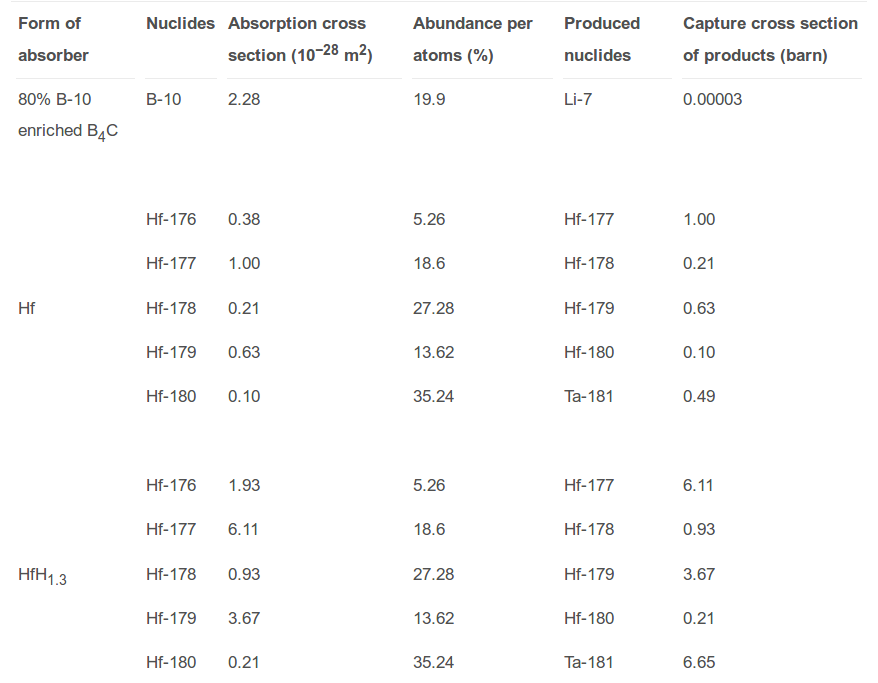
\includegraphics[scale=0.23]{./images/axs.png}
  \end{center}
  \caption{Absorption cross section comparison of various forms}
  \label{fig:axs}
\end{figure}

\end{frame}

\begin{frame}
\frametitle{Hafnium as an absorber - 2/3}
Continued absorption integrity and low induced radioactivity after irradiation.

\begin{figure}[htbp!]
  \begin{center}
      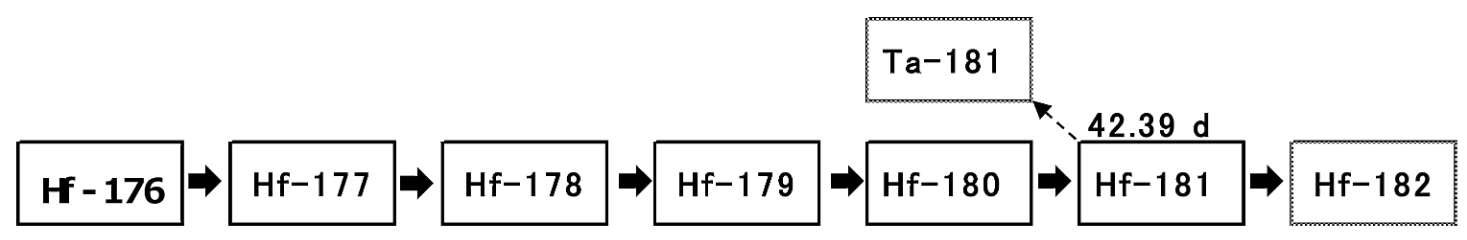
\includegraphics[scale=0.2]{./images/decay_chain.png}
  \end{center}
  \caption{Nuclear transmutation of hafnium nuclides by capture. Ta-181 is stable and Hf-182
            has a half life of 8.9e6 years}
  \label{fig:dec}
\end{figure}
\end{frame}

\begin{frame}
\frametitle{Hafnium as an absorber - 3/3}
Other peripheral beneficial characteristics of hafnium include:
\begin{itemize}
  \item Malleability, ductility
  \item Rich reserve of raw materials
  \item Resistance to chemical activity
  \item Corrosion resistance
  \item High melting temperature
  \item Stable at high temperature and pressure
\end{itemize}
\end{frame}

\begin{frame}
\frametitle{Objectives}
Demonstrate the feasibility and benefits of using a \hfh control rod
over a \bc control rod in a \gls{JSFR} by comparing various metrics.
Metrics include:
\begin{itemize}
    \item Reactor nuclear characteristic ( Enrichment, Na void reactivity, etc.)
    \item Coolant flow rate
    \item Hydrogen desorption
    \item Control rod performance over time (irradiation)
    \item Linear heat rate
    \item Reactivity
    \item Temperature distribution
\end{itemize}
\end{frame}


\section{Methodology}


\begin{frame}
\frametitle{Previous Work}
6-year study of \hfh control rod feasibility
\begin{figure}[H]
\centering
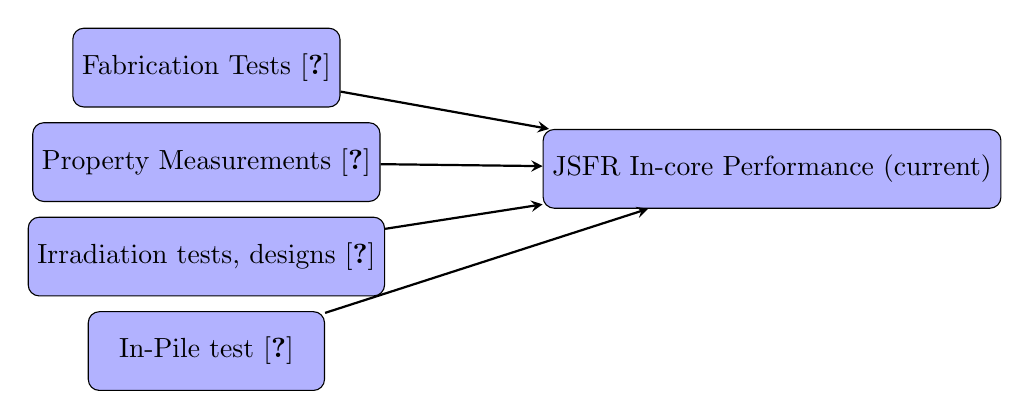
\begin{tikzpicture}[node distance=1.2cm]
\node (fab) [process] {Fabrication Tests \cite{konashi_study_2010}};
\node (pro) [process, below of=fab] {Property Measurements \cite{konashi_utilization_2010}};
\node (irr) [process, below of=pro]{Irradiation tests, designs \cite{konashi_environmentally_2012}};
\node (inp) [process, below of=irr]{In-Pile test \cite{hirai_study_2010}};
\node (core) [process, above right=0.1cm and 2cm of irr] {\gls{JSFR} In-core Performance (current)};

\draw [arrow] (fab) -- (core); 
\draw [arrow] (inp) -- (core);
\draw [arrow] (irr) -- (core);
\draw [arrow] (pro) -- (core);
\end{tikzpicture}
\end{figure}

\end{frame}


\begin{frame}
\frametitle{Deterministic Method for reactor design}
\begin{itemize}
\item Unified 70-group fast set of group constants (ADJ2000R) \cite{hazama_development_2002}
\item Diffusion Code (TRISTAN)
  \begin{itemize}
    \item verified with (CITATION) from \gls{ORNL}.
  \end{itemize}
\item Perturbation Code (TRI-PERT) 
  \begin{itemize}
  \item nuclear characteristics
  \end{itemize}
\item Depletion (JFS3-J3.3)
\item Heating density of hafnium hydride absorber (MCNP-5) \cite{mcnp_monte_2003}
\item Nuclear Data (ENDL92 for Hf and ENDF-VI for others)
\end{itemize}
\end{frame}

\begin{frame}
\frametitle{Monte Carlo Method}
\begin{itemize}
    \item Effects of reactor constants and heterogeneity of control rod structure (MVP, GMVP) \cite{nagaya_mvp/gmvp_2005}  
    \begin{itemize}
        \item Neutron and photon transport
        \item Based on continuous energy and multigroup methods
    \end{itemize}
\end{itemize}
\end{frame}



\begin{frame}
\frametitle{Core simulation with hafnium control rods}
Hafnium hydride control rods replaced the boron carbide in the
\gls{JSFR} \cite{ogura_conceptual_2009} for comparison, with U-TRU mixed oxide fuel \cite{ikeda_application_2014}.
\begin{figure}[htbp!]
  \begin{center}
      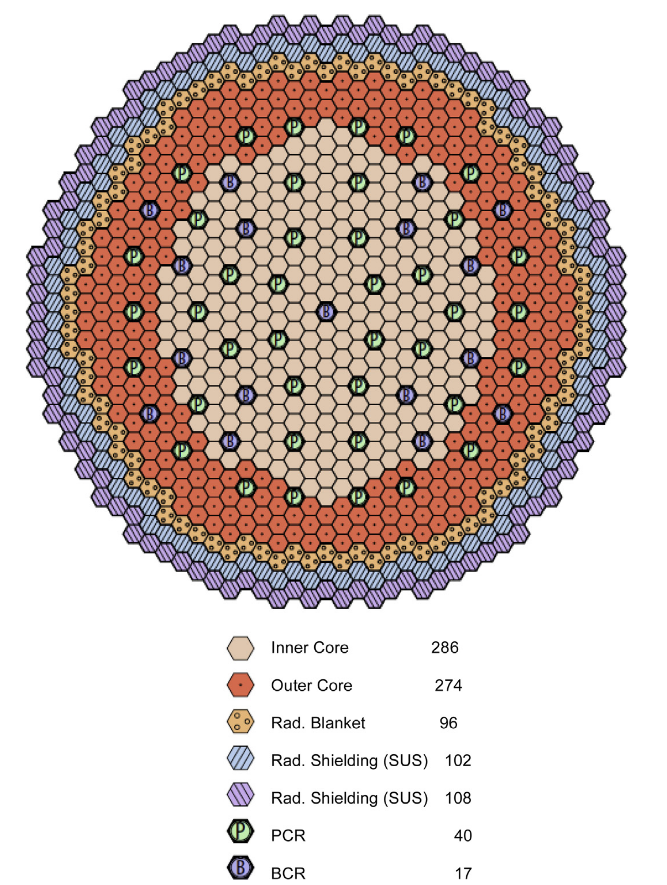
\includegraphics[scale=0.15]{./images/core.png}
  \end{center}
  \caption{Core diagram of the \gls{JSFR}.}
  \label{fig:core}
\end{figure}
\end{frame}

\begin{frame}
\frametitle{Assumptions}
\begin{itemize}
    \item Pu enrichments so that excess reactivity \textasciitilde 0.2\% 
    \item ratio of H to Hf is constant (no hydrogen desorption)
    \item Transmutation from Hf-180 to Hf-181, or Ta-181 neglected.
    \item temperature of cladding limited to 600$^\cdot$C
    \item Absorber pellet limited $800^\cdot$C for hydrogen desorption
    \item No swelling of \hfh control rod
\end{itemize}
\end{frame}

\begin{frame}
\frametitle{Control Rod Location}
\begin{figure}[htbp!]
  \begin{center}
      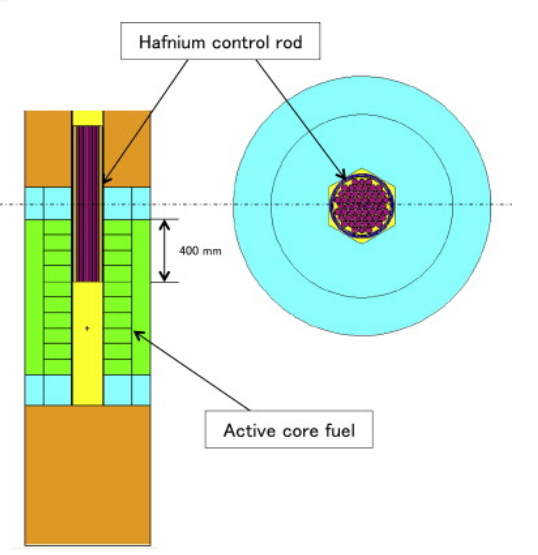
\includegraphics[scale=0.3]{./images/elevator.png}
  \end{center}
  \caption{Elevator view of control rod position with respect to active core fuel. Control rod remains static.}
  \label{fig:elev}
\end{figure}
\end{frame}


\section{Results}



\begin{frame}
\frametitle{Reactivity of \hfh control rods}
Reactivity similar to 80\% B-10 enriched boron carbide rods with
enhanced control rod reactivity with hydrogen moderation of neutrons.
\begin{figure}[htbp!]
  \begin{center}
      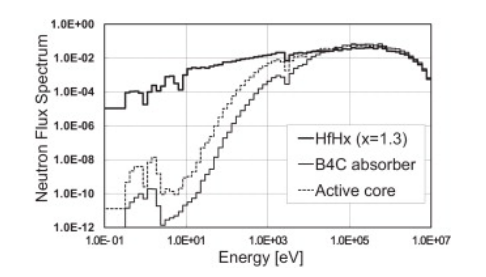
\includegraphics[scale=0.5]{./images/spectrum.png}
  \end{center}
  \caption{Neutron spectrum of the hafnium hydride control rod}
  \label{fig:spec}
\end{figure}
\end{frame}

\begin{frame}
\frametitle{\hfh control rod depletion calculation results - 1/2}
Neutron absorption performance degrades very little with irradiation
because the produced isotopes are also absorbers.
\begin{figure}[htbp!]
  \begin{center}
      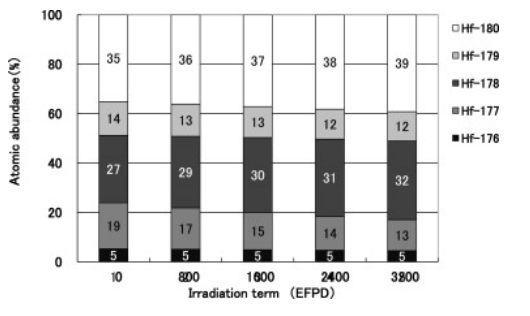
\includegraphics[scale=0.48]{./images/irrad_isotope.png}
  \end{center}
  \caption{Change of hafnium isotope ratio in the control rod during irradiation.}
  \label{fig:irrad_iso}
\end{figure}
\end{frame}

\begin{frame}
\frametitle{\hfh control rod depletion calculation results - 2/2}
Reactivity degradation is 4\% after 2400 \gls{EFPD} ( 3 cycles )
\begin{figure}[htbp!]
  \begin{center}
      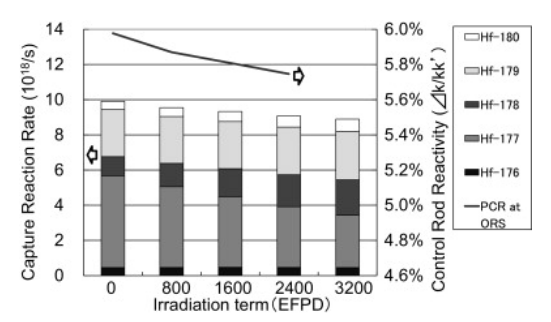
\includegraphics[scale=0.4]{./images/irrad_reac.png}
  \end{center}
  \caption{Capture reaction rate and reactivity of hafnium hydride control rod.}
  \label{fig:irrad_reac}
\end{figure}
\end{frame}

\begin{frame}
\frametitle{Results of nuclear calculation with \hfh control rods}
Nuclear characteristics as good as or better than with \bc.
\begin{figure}[htbp!]
  \begin{center}
      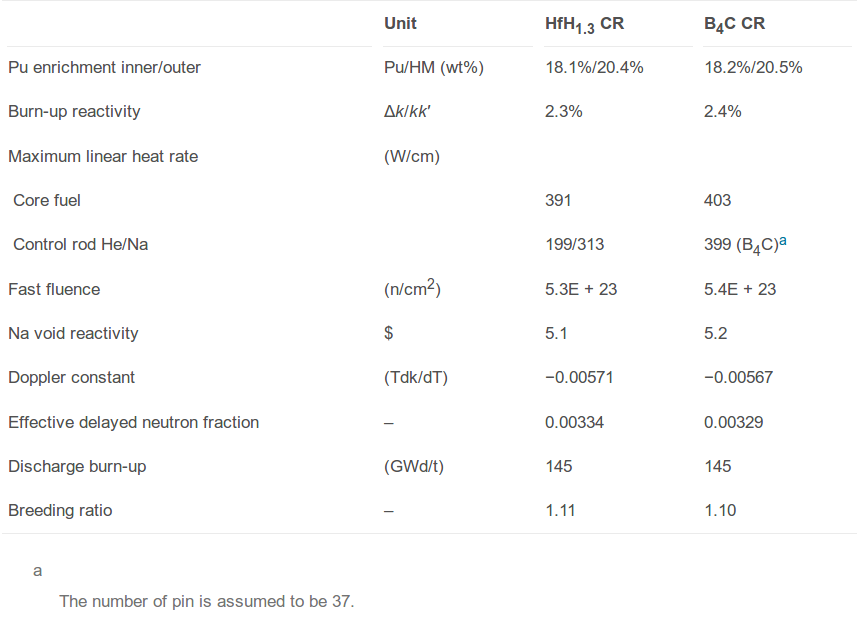
\includegraphics[scale=0.25]{./images/reac.png}
  \end{center}
  \caption{Nuclear characteristics of the reactors with the hafnium hydride and the boron carbide absorber.}
  \label{fig:reac}
\end{figure}
\end{frame}


\begin{frame}
\frametitle{Heat profile in \hfh  control rod}
Neutron-induced energy of the absorber is approximately twice as large as \bc.
Limit of 800$^\circ$C to prevent hydrogen desorption.
Maximum absorber temperature = 718$^\circ$C
\begin{figure}[htbp!]
  \begin{center}
      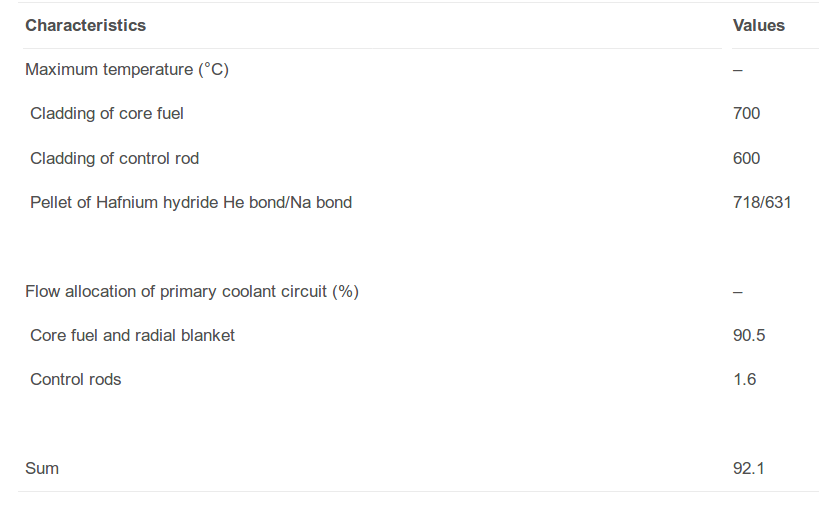
\includegraphics[scale=0.28]{./images/th.png}
  \end{center}
  \caption{Thermal hydraulic characteristics in the hafnium hydride control rod deployed reactor.}
  \label{fig:th}
\end{figure}
\end{frame}


\begin{frame}
\frametitle{Heat density of \hfh}
Twice the heat generation of \bc, but peak of heat densities are comparable
due to hydrogen moderation and gamma-ray transport.
\begin{figure}[htbp!]
  \begin{center}
      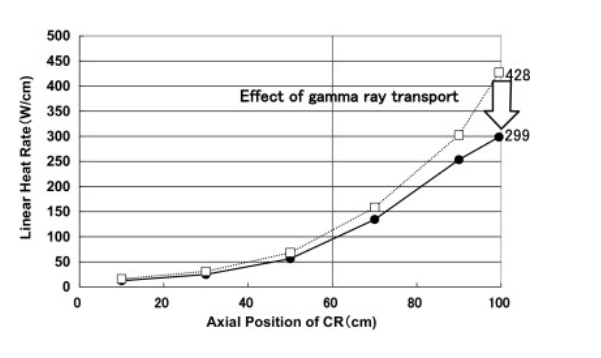
\includegraphics[scale=0.3]{./images/gamma.png}
  \end{center}
  \caption{Effect of gamma transport in the linear heat rate of \hfh absorber.}
  \label{fig:reac}
\end{figure}
\end{frame}

\begin{frame}
\frametitle{Local radial power distribution of subassembly adjacent to control rod}
\bc: Less power near the control rod

\hfh: More power near the control rod due to hydrogen moderation leading
to enhanced reaction rate.

\begin{figure}[htbp!]
  \begin{center}
      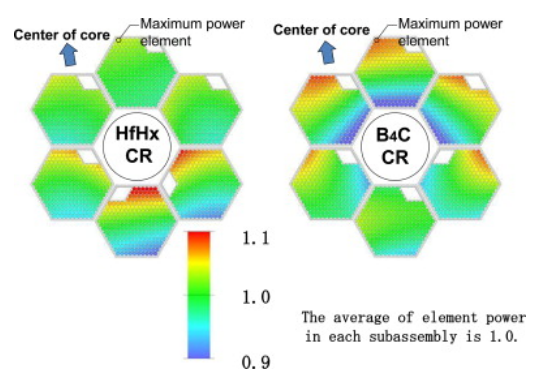
\includegraphics[scale=0.3]{./images/local.png}
  \end{center}
  \caption{Local radial power distribution of subassembly adjacent to control rod inserted.}
  \label{fig:local}
\end{figure}
\end{frame}

%%%%%%%%%%%%%%%%%%%%%%%%%%%%%%%%%%%%%%%%%%%%%%%%%%5
\iffalse

\begin{frame}
\frametitle{Design requirements of \gls{SFR}}
    \begin{table}[h]
      \centering 
      \begin{tabularx}{\textwidth}{mb}
      \hline
      Requirement & Benefit from using \hfh \\ 
      \hline
      Intrinsic negative feedback &     \\ 
      Na void reactivity $\leq$ \$6 & \$5.1\\ 
      Coolant flow &  8\% less at cladding temperature limit  \\
      Shutdown abilities &  \\ 
      Hydrogen desorption & future work\\ 
      Off-normal events & future work \\ 
      \hline
      \end{tabularx}
      \caption {Benefits of using \hfh in \gls{SFR} relative to \bc}
      \label{tab:ben}
    \end{table}
\end{frame}
\fi
%%%%%%%%%%%%%%%%%%%%%%%%%%%%%%%%%%%%%%%%%%%%%%%%

\begin{frame}
\frametitle{Important Results and Conclusion}
\begin{itemize}
  \item Longer lifetime due to hafnium isotopes after neutron absorption
  \item Hydrogen increase of absorption
  \item 9 years lifetime (compared with 1-2 year for \bc)
  \item Slightly better reactor parameters (flow rate, safety margin, breeding ratio etc.)
  \item Able to meet absorber temperature below hydrogen desorption temperature
\end{itemize}
\end{frame}

\section{Assessment}


\begin{frame}
\frametitle{Relevance and Novelty}
\begin{itemize}
  \item Reactor performance metric change with control rod
  \item Improvements on \gls{SFR} design
  \item Improvements on control rod lifetime and performance
  \item Reduction in low-level waste
    \begin{itemize}
        \item Less radiotoxicity from used control rods
        \item Longer lifetime = less waste
    \end{itemize}
\end{itemize}
\end{frame}

\begin{frame}
\frametitle{Technical Detail and Analytic Rigor}
\begin{itemize}
    \item Reactivity and `nuclear characteristics' of \gls{JSFR}
    \item Thermal profile of reactor and control rod
    \item Lacking in transient scenarios
\end{itemize}
\end{frame}


\begin{frame}
\frametitle{Verifiability (Reproducibility)}
\begin{itemize}
  \item Codes are well-known and published
  \item Input files unavailable
  \item Specifications of simulation (geometry, pellet diameter etc.) well-documented.
\end{itemize}
\end{frame}


\begin{frame}
\frametitle{Clarity}
\begin{itemize}
  \item Grammatical mistakes 
  \item Confusing noun-verb relationship
  \item Run-on sentences ("Futhermore the comparison with the B-10 enriched boron carbide rods.")
  \item Lengthy explanation would be much more concise in tables.
  \item Abstract represents the conclusion well.
  \item Axial location of control rod in core simluation unclear
\end{itemize}
\end{frame}


\begin{frame}
\frametitle{Technical Gaps, missing analyses}
\begin{itemize}
    \item Multiplication factor (assuming critical because it is a control rod experiment)
    \item Assumed static control rod position for entire cycle
    \item Non-normal operation scenarios
    \begin{itemize}
        \item Large temperature shift effect
        \item Hydrogen desorption
        \item Loss of hydrogen leads to lower control rod worth
    \end{itemize}
    \item Swelling of hafnium hydride
    \item Flux profile of reactor
    \item Static control rod position
    \begin{itemize}
        \item Axial variation of control rod depletion
    \end{itemize}
    \item What happens when Hf-180 absorbs a neutron?
    \item Effect of higher power near control rod
\end{itemize}
\end{frame}

\section{Extension}


\begin{frame}
\frametitle{Future Work suggested by authors}
\begin{itemize}
  \item Hydrogen desorption in operating conditions
  \item Uncertainty of control rod reactivity
  \item Swelling of control rod
\end{itemize}
\end{frame}


\subsection{Potential extensions of current work }
\begin{frame}
\frametitle{Potential extension of work}
\begin{itemize}
  \item Accident scenarios
    leading to higher core temperature $\rightarrow$ desorption of hydrogen $\rightarrow$ less control rod worth
  \item Axial depletion change during operation
  \begin{itemize}
      \item Position of control rod changes over time with operation
      \item Axial variation of irradiation / depletion
  \end{itemize}
  \item With the allowance of longer life control rods, 'breed and burn'
  core designs with a much longer cycle time of 800 EFPD
  \item Swelling of control rod with longer irradiation
  \item Effect of local moderation on used fuel composition and flux
  \item Effect of higher power near \hfh control rod
  \item Enrichment of Hf (increase composition of lower isotopes) for better performance
\end{itemize}
\end{frame}

\subsection{Extension 1 - Accident Scenario and Hydrogen Desorption}

\begin{frame}
\frametitle{Extension 1 - Accident Scenarios}
An accident scneario where the temperature of the core increases beyond operating tempearture
and the control rods are dropped to high temperature sodium / fuel 
\begin{itemize}
    \item Hydrogen desorption possible at 1,000$^\cdot$C \cite{konashi_development_2013}
    \item Core temperature higher than 1,000$^\cdot$C during accident scenarios
    \item \hfh can lose up to 65\% of reactivity with hydrogen loss
\end{itemize}
\end{frame}


\begin{frame}
\frametitle{Preliminary study}
\begin{enumerate}
    \item \hfh in higher temperature than 800$^\cdot$C and observe hydrogen desorption with temperature
    \item Calculate model for hydrogen desorption with temperature
    \item Calculate \hfh control rod reactivity change with temperature / irradiation
\end{enumerate}
\end{frame}

\begin{frame}
\frametitle{In-core Simulation}
\begin{enumerate}
    \item Run accident scenario core simulation with implemented hydrogen desorption
          model
    \item Modify cross section of control rod with temperature / irradiation using model obtained
    \item Track core nuclear and thermal metrics with time
    \item Identify reactor shutdown problems
\end{enumerate}
\end{frame}

\subsection{Extension 2 - Axial Variation of Control Rod}

\begin{frame}
\frametitle{Extension 2 - Axial variation of control rod}
In normal operation control rod position moves within cycle.
\begin{itemize}
    \item This paper remains control rod static at half way pulled out
    \item In reality control rod would be irradiated more if starting from bottom
    \item Axial variation of control rod depletion
\end{itemize}
\end{frame}


\begin{frame}
\frametitle{Methods to measure control rod movement in cycle}
Simplified to more elaborate:
\begin{itemize}
  \item Linear control rod position from bottom to top throughout cycle ($y = \frac{h}{800}t $)
  \item Past historical control rod movement throughout cycle
  \item Use code to figure out critical rod position in t
\end{itemize}
\end{frame}


\begin{frame}
\frametitle{Axial power distribution change with control rod depletion}
Run core simulation with control rod movement.
\begin{itemize}
    \item Core axial power distribution with axially-varying control rod
    \item Linear heat rate with axially-varying control rod
    \item Control rod depletion
\end{itemize}
\end{frame}

\section{Conclusion}
\begin{frame}
\frametitle{Conclusion}
\begin{itemize}
    \item This paper claims feasibility of \hfh control rods in \gls{SFR} reactors
    \item Performs as good as or better in a \gls{JSFR} than \bc control rods using the methodology by the authors
    \item Multiple issues have not been taken into account
    \item Hydrogen desorption, criticality and swelling of control rod requires further study
\end{itemize}
\end{frame}

%%--------------------------------%%
%%--------------------------------%%
\begin{frame}[allowframebreaks]
  \frametitle{References}
  \bibliographystyle{abbrv}
  {\footnotesize \bibliography{bibliography} }
\end{frame}

%%--------------------------------%%


\begin{frame}
\frametitle{Coolant Cross section}
\begin{figure}[htbp!]
  \begin{center}
      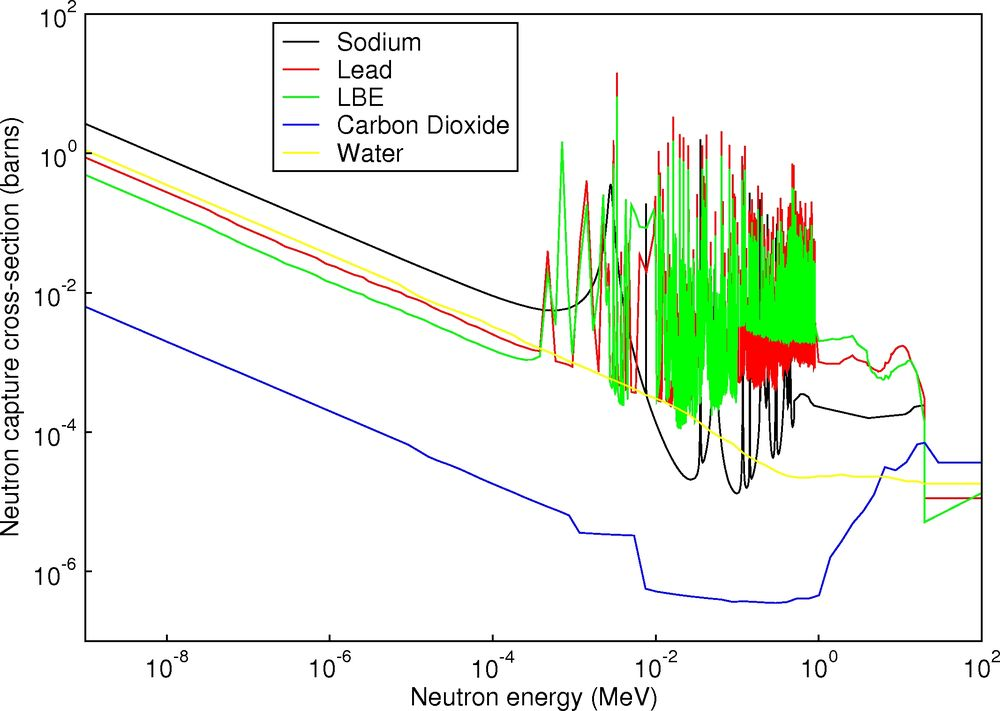
\includegraphics[scale=0.7]{./images/coolant.jpg}
  \end{center}
  \caption{Coolant and cross section \cite{stacey_nuclear_2007}}
  \label{fig:reac}
\end{figure}
\end{frame}


\begin{frame}
\frametitle{Cheat Sheet}
\begin{itemize}
  \item Reactor Shutdown System - passively released due to curie point effect by abnormal rising of coolant temperature.
  \item Passive safety $\rightarrow$ thermal expansion of absorbing liquid
  \item Edge - Na expansion leads to more neutron leakage (negative reactivity coeff)
  \item Center - Na expansion leads to less absorption (positive reactivity coeff)
  \item Doppler coefficient : "Fuel temperature coefficient of reactivity" how reactivity changes per temperature in fuel
  \item Gamma Ray transport: Gamma ray has a long mfp that the decay energy to leave the zone of origin
  \item Fuel Slumping: Fuel melts to the bottom of the pin, increasing fuel density
  \item Peaking Factor: $\frac{Highest Local Power Density}{Avg Power Density}$
\end{itemize}
\end{frame}


Predictor - corrector

Current flux, deplete the fuel, if it is critical
Run another calculation to finds

ENDF JEFF 252 groups 'continuous'


SERPENT 2 and SCALE are for doing depletion calculation
generates homogenized cross section
collapses to 7 group for fast


homogenized cross sections to characterize the core
  criticality values
  critcial control rod position / ppm for boron
  fuel depletion

Thermal-hydraulics code
internal to PARCS
coupled to TRACE

Provide reduced number of groups of cross sections to
Core simulators like PARCS, set delta t
adjust critical boron concentration and control rod position.


\end{document}



